Git est hébergeur de code, de projet, qui permet d'avoir accès à ceux-ci n'importe où il y a internet.
Il s'utilise avec des systèmes de branches et s'utilise à la le plus souvent console, mais nous l'avons utiliser aussi avec Gitg, qui est une interface qui permet d'avoir un visuel des branches (Voir ~\ref{gitg} page~\pageref{gitg}).


\begin{figure}[h]
\caption{\label{gitg} Capture de Gitg}
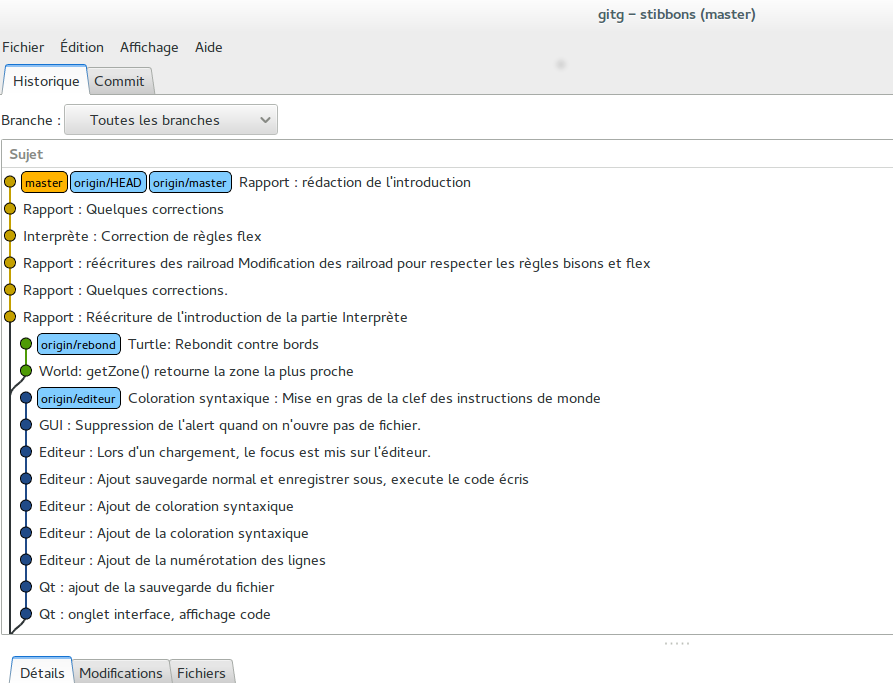
\includegraphics[scale=0.35]{doc/report/uml/gitbranche.png}
\end{figure}


Les commandes commence toujours par git :
\begin{itemize}
\item git checkout nom-branche, permet de changer de branche,
\item git branch, de savoir sur quel branche on est,
\item git add fichiers, permet de suivre des fichiers (enregistrer les modifications qu'on fait sur des fichiers),
\item git commit, permet de commiter les changements des fichiers qu'on suit,
\end{itemize}


De plus, Git permet sur son site de déclarer des \enquote{issues}. Ce sont des problèmes à corriger.

